\item\subquestionpoints{15}
\textbf{[Coding Problem] K-Means Compression Implementation.}
From the \texttt{data} directory, open an interactive Python prompt, and type
%
\begin{center}
  \texttt{from matplotlib.image import imread; import matplotlib.pyplot as plt;}
\end{center}
%
and run \texttt{A = imread('peppers-large.tiff')}. Now, \texttt{A} is a ``three
dimensional matrix,'' and \texttt{A[:,:,0]}, \texttt{A[:,:,1]} and
\texttt{A[:,:,2]} are 512x512 arrays that respectively contain the
red, green, and blue values for each pixel. Enter {\tt plt.imshow(A); plt.show()} to
display the image.

Since the large image has 262144 pixels and would take a while
to cluster, we will instead run vector quantization on a smaller
image. Repeat (a) with {\tt peppers-small.tiff}.  Treating each
pixel's $(r, g, b)$ values as an element of $\Re^3$, run K-means\footnote{
Please implement K-means yourself, rather than using built-in functions.}
with 16 clusters on the pixel data from this smaller image,
iterating (preferably) to convergence, but in no case for less than
30 iterations. For initialization, set each cluster centroid to the
$(r, g, b)$-values of a randomly chosen pixel in the image.

Take the matrix \texttt{A} from \texttt{peppers-large.tiff}, and
replace each pixel's $(r, g, b)$ values with the value of the closest
cluster centroid. Display the new image, and compare it visually to
the original image. \textbf{Include in your write-up all your code and a copy of your
compressed image.}

\ifnum\solutions=1 {
  \begin{answer}

Code is as follows
    \lstinputlisting[language=Python]{files/p05_kmeans.py}

    Please see Figure \ref{fig:compressed} for the compressed image.

    \begin{figure}[htbp]
        \centering
        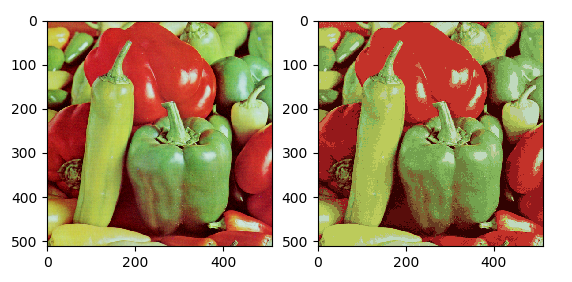
\includegraphics[width=0.7\linewidth]{pics/compressed.png}
        \caption{Compressed}
        \label{fig:compressed}
    \end{figure}
\end{answer}

} \fi
